\documentclass[a6paper,10pt]{article}
%\usepackage[T1]{fontenc}
\usepackage[british]{babel}
\usepackage[utf8]{inputenc}
\usepackage{float, graphicx,amsmath,amsfonts,cite,enumerate,caption,subcaption}
\usepackage[final]{pdfpages}
\usepackage{wrapfig}
\usepackage[margin=0.3in]{geometry}
\usepackage{sidspaltHack}
\usepackage{digital}


\setlength{\oddsidemargin}{-0.37in}
\setlength{\textwidth}{215pt}

\pagestyle{empty}


% TODO: Varför är inte det här i alfa-kapitlet?
\begin{document}
\nysida{2}{}\noindent
9. Gyckel bör framföras åtminstone av varje grupp på festen. Exempel på grupper är nämnder, föreningar, festlag, n$\emptyset$llegrupp o.d. \\Ett dåligt gyckel är likväl ett gyckel och förtjänar att representeras som sådant.
\vspace{5pt} \\
10. En bör inte lämna bordet innan taffeln bryts, vanligtvis med 'O Gamla Klang' eller 'Sista Punschvisan'. Naturligtvis är kortare uppbrott för besök i baren eller sminkrummet fullt acceptabla.\vspace{5pt}   
11. Visa uppskattning gentemot festfixarna så att de vill arrangera fler fester. Fjäsk går hem.
\vspace{5pt} \\
12. I den mån det är möjligt, bör festdeltagarna sjunga samma sång som toastmastern. Att sjunga starkt är att sjunga vackert.
\vspace{5pt} \\
13. Anarkisång får bara förekomma om toastmastern är för långsam eller glömmer sånger av allmänt intresse.\\ Denna regel skall nyttjas ytterst varsamt. Framför allt av de som inte själva arrangerat fester eller toastmastrat.
\vspace{5pt} \\
14. Ha roligt, men glöm inte - \textit{force odeur} ser allt.
\vspace{-11pt}
\vspace{5pt}   \\
15. Under bordet råder högertrafik. Trafik på bordet undanbedes. Utropet "N.N. på bordet" betyder att N.N. ska ställa sig på stolen, och att en kan ha hamnat med gymnasieelever.
\vspace{5pt} \\
16. Intagen mat och dryck återtages ej.
\vspace{5pt} \\
17. Antalet regler skall vara 17.

\nysida{2}{1}
\setlength{\oddsidemargin}{-0.47in}
\noindent
\chaptertitle{B$\beta$}{Visor till gasque}
\small
\begin{center}
   \songtitle{$\beta1$}{Porthos visa (Athos visa)}
   \mel{You can't get a man with a gun}
   \sheetmusicnoticenormal{Noter finns i notkapitlet}
\end{center}
\begin{lyrics}
Jag vill börja gasqua, var fan är min flaska?\\
Vem i helvete stal min butelj?\\
Skall törsten mig tvinga, en TT börja svinga\\
Nej, för fan bara blunda och svälj\\
Vilken smörja, får jag spörja\\
"Vem för f-n tror att jag är en älg?"\\
 \newline
Till England vi rider och sedan vad det lider\\
Träffar vi välan på någon pub\\
Och där skall vi festa, blott dricka av det bästa\\
Utav Whisky och portvin, jag tänker gå hårt in\\
För att prova på rubb och stubb
\end{lyrics}
\auth{Bergsspexet 1960}
%
%\begin{figure}[!h]
%\centering
%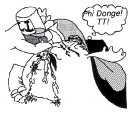
\includegraphics[width=0.3\textwidth]{jagvillborjagasqua.png}
%\end{figure}

\nysida{2}{2}
\setlength{\oddsidemargin}{-0.37in}
\begin{center}
\songtitle{$\beta2$}{Lyft ditt välförsedda glas}
   \mel{Ding dong, merrily on high} 
   \sheetmusicnoticenormal{Noter till blandad kör finns i notkapitlet}
\end{center}
\begin{lyrics}
Lyft ditt välförsedda glas, \\
det är en ljuvlig börda! \\
Nu har polarna kalas, \\
i morgon är det lördag! \\
$\|$: Dingedingedinge dingedingedinge \\
Dingedingedinge ding dong dong \\
Vi segern snart skall skörda. :$\|$ \\
\newline
Sätt nu glaset till din mun, \\
se döden på dig vänta! \\
Nu har polarna kalas, \\
hör liemannen flämta! \\
$\|$: Dingedingedinge dingedingedinge \\
Dingedingedinge ding dong dong \\
Begravningsklockor klämta. :$\|$
\end{lyrics}

\begin{figure}[!h]
\hfill
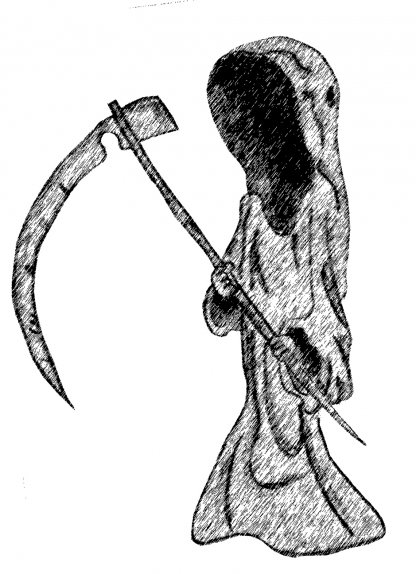
\includegraphics[width=0.4\textwidth]{liemannen.jpg}
\end{figure}

\nysida{2}{3}
\setlength{\oddsidemargin}{-0.47in}
\begin{center}
   \songtitle{$\beta3$}{Härjavisan}
   \mel{Gärdebylåten}
\end{center}
\begin{lyrics}
Hurra nu ska en äntligen \\få röra på benen,\\
hela stammen jublar \\och det spritter i grenen.\\
Tänk att än en gång få spränga fram \\på Brunte i galopp.
\vspace{5pt}\\
Din doft o kära Brunte är \\trots brist i hygienen\\
för en vild mongol\\ minst lika ljuv som syrenen.\\
Tänk att på din rygg få rida runt \\i stan och spela topp! 
\vspace{5pt}\\
\textbf{Ja, nu skall vi ut och härja\\
supa och slåss och svärja,\\
bränna röda stugor,\\
slå små barn och säga fula ord\\
Med blod ska vi stäppen färga\\
nu änteligen lär jag\\
kunna dra nån riktig nytta \\
av min Hermodskurs i mord. }
\vspace{5pt}\\
Ja, mordbränder är klämmiga, \\ta fram fotogenen\\
eftersläckningen tillhör just de fenomenen,\\
inom brandmansyrket \\som jag tycker det är nån nytta med.
\newpage 
\setlength{\oddsidemargin}{-0.37in}
\noindent
Jag målar för mitt inre upp \\den härliga scenen\\
blodrött mitt i brandgult, \\ej ens prins Eugen, en\\
lika mustig vy kan måla, \\ens om han målade med sked.
\vspace{5pt}\\
\textbf{Ja, nu skall vi ut och härja...} 
\vspace{5pt}\\
Liksom våra fäder, \\
vikingarna i Norden\\
drar vi riket runt \\och super oss under borden.\\
Brännvinet har blivit \\ett elixir för kropp såväl som själ.
\vspace{5pt}\\
Känner du dig liten \\och är ynklig på jorden\\
växer du med supen \\och blir stor uti orden,\\
slår dig för ditt stolta bröst \\och blir då värdig från hår till häl. 
\vspace{5pt}\\
\textbf{Ja, nu skall vi ut och härja...}
\end{lyrics}
\auth{Text: Hans Alfredsson \\Lundaspexet Djingis Khan 1954}
\vspace{-30pt}
\begin{figure}[!h]
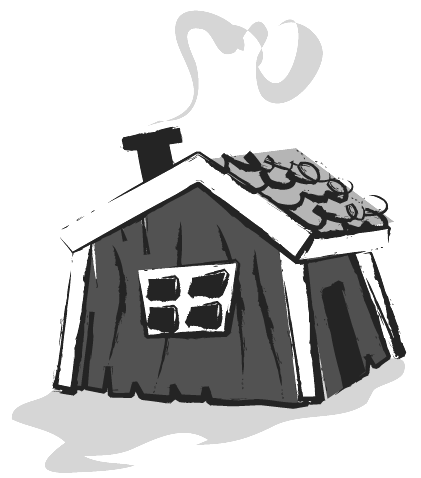
\includegraphics[width=0.32\textwidth]{rodstuga.png}
\end{figure}

\nysida{2}{4}
\setlength{\oddsidemargin}{-0.47in}
\begin{center}
   \songtitle{$\beta4$}{Kalmarevisan}
   \small{\textit{Försångare/\textbf{Alla}\\Sjungs lämpligen på småländska.}}
\end{center}
\begin{figure}[!h]
\begin{subfigure}{0.55\textwidth}
\small Uti Kalmare stad\\
ja där finns det ingen kvast\\
\textbf{förrän lördagen!}
\vspace{5pt}\\
\textit{Hej dick... \\
\textbf{...hej dack!}\vspace{5pt} \\
Jag slog i...\\
\textbf{...och vi drack!}}
\end{subfigure}
\begin{subfigure}{0.41\textwidth}
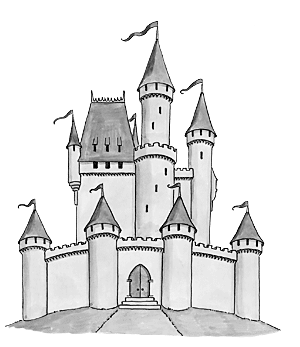
\includegraphics[width=0.9\textwidth]{kalmarslott3.png}
\end{subfigure}
\end{figure}
\vspace{-5pt}
\textit{Hej dickom dickom dack!\\
\textbf{Hej dickom dickom dack!}}\vspace{5pt} \\
\textbf{För uti Kalmare stad,\\ ja där finns det ingen kvast\\ förrän lördagen!}
\vspace{5pt} \\
$\|$: När som bonden kommer hem \\
\textbf{kommer bondekvinnan ut :$\|$ \\och är så stor i sin trut.}
\vspace{5pt} \\
\textit{Hej dick...} (etc.) 
\vspace{5pt} \\
$\|$: Var är pengarna du fått?\\
\textbf{Jo, dem har jag supit opp:$\|$ \\uppå Kalmare slott}
\vspace{5pt} \\
\textit{Hej dick...} (etc.)
\vspace{5pt} \\
$\|$:Jag skall mäla dig an\\
\textbf{för vår kronbefallningsman :$\|$ \\ och du skall få skam.}
\nysida{2}{5}
\setlength{\oddsidemargin}{-0.37in}
\noindent
\vspace{5pt} \\
\textit{Hej dick...} (etc.)
\vspace{5pt} \\
$\|$: Kronbefallningsmannen vår \\
\textbf{satt på krogen i går:$\|$\\ och var full som ett får.}
\vspace{5pt} \\
\textit{Hej dick...} (etc.)

% TODO: Framöver bör kalmarevisan läsas av maskinellt från originalet,
% trots den tunga formateringen.
% Versionen nedan används enbart av den digitala sångboken.
\begin{comment}@digitallyrics
F: Uti Kalmare stad\\
ja där finns det ingen kvast\\
A: förrän lördagen!\\
\\
F: Hej dick...\\
A: ...hej dack!\\
F: Jag slog i...\\
A: ...och vi drack!\\
F: Hej dickom dickom dack!\\
A: Hej dickom dickom dack!\\
För uti Kalmare stad, ja där finns det ingen kvast förrän lördagen!\\
\\
||: F: När som bonden kommer hem\\
A: kommer bondekvinnan ut :|| och är så stor i sin trut.\\
\\
F: Hej dick...\\
\\
||: F: Var är pengarna du fått?\\
A: Jo, dem har jag supit opp :|| uppå Kalmare slott\\
\\
F: Hej dick...\\
\\
||: F: Jag skall mäla dig an\\
A: för vår kronbefallningsman :||  och du skall få skam.\\
\\
F: Hej dick...\\
\\
||: F: Kronbefallningsmannen vår\\
A: satt på krogen i går :|| och var full som ett får.\\
\\
F: Hej dick...
\end{comment}
\begin{center}
   \songtitle{$\beta5$}{Jag skall festa}
\mel{Bamse-låten}
\end{center}
\begin{lyrics}
Jag skall festa, ta det lugnt med spriten,\\
ha det roligt utan att va' full.\\
Inte krypa runt med festeliten,\\
ta det sansat för min egen skull.
\vspace{5pt} \\
Först en öl i torra strupen,\\
efter det så kommer supen,\\
i med vinet, ned med punschen\\
sist en groggbuffé.
\vspace{5pt} \\
Jag är skitfull, däckar först av alla,\\
missar festen, men vad gör väl de'.\\
Blandar hejdlöst öl och gammal filmjölk,\\
kastar upp på bordspartnern bredve'.
\vspace{5pt} \\
Först en öl i torra strupen...
\vspace{5pt} \\
Spyan rinner ner för ylleslipsen,\\
raviolin torkar i mitt hår.\\
Vem har lagt mig här i pissoaren,\\
vems är gaffeln i mitt högra lår?
\end{lyrics}

\nysida{2}{6}
\setlength{\oddsidemargin}{-0.47in}
\begin{center}
   \songtitle{$\beta6$}{Emils spritvisa}
   \mel{Snickerboa}
\end{center}
\begin{lyrics}
Till spritbutiken ränner jag \\
och bankar på dess port. \\
Jag vill ha nå't som bränner bra \\
och gör mig skitfull fort. \\
Expediten sa: "Godda', \\
hur gammal kan min herre va'? \\
Har du nå't leg, ditt jävla drägg?\\ 
Kom hit igen när du fått skägg!" \\
\newline
Men detta var ju inte bra \\
jag vill bli full i kväll. \\
Då plötsligt en idé fick jag: \\
de har ju sprit på Shell! \\
Många flaskor stod där på rad \\
så nu kan jag bli skitfull och glad.\\ 
Den röda vätskan rinner ner... \\
Nu kan jag inte se nå't mer. 
\end{lyrics}

\nysida{2}{7}
\setlength{\oddsidemargin}{-0.37in}
\begin{center}
   \songtitle{$\beta7$}{Hej på er vänner alla}
\end{center}
\begin{lyrics}
Hej på er vänner alla, \\
ja vi ska supa tills dess vi falla, \\
och brännvinslitern, den är för liten, \\
den är för liten för oss alla! \\
\newline
Och en gång när jag är döder\\ 
och lagd mellan tvenne vänner. \\
Begrav mig, begrav mig \\
i en brännvinskällare på Söder. \\
\newline
Och på min gravsten skall det stå ristat \\
med tvenne små enkla rader: \\
"Här vilar det en fylletrogen, \\
som alltid var så glad och goder.\\ 
Här vilar det en fylletrogen, \\
som alltid var så glad och goder." 
\end{lyrics}
\vspace{35pt} \\
\begin{figure}[!h]
\centering
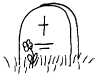
\includegraphics[width=0.5\textwidth]{gravsten.jpg}
\end{figure}

\nysida{2}{8}
\setlength{\oddsidemargin}{-0.47in}
\begin{center}
   \songtitle{$\beta8$}{Lille Olle}
   \mel{Katyuscha}
\end{center}
\begin{lyrics}
Lille Olle skulle gå på disco, \\
men han hade inte någon sprit.\\ 
Lille Olle skaffa' lite hembränt, \\
lille Olle gick då på en nit. \\
\newline
La lalla la la la ... \\
\newline
Lille Olle skulle börja festa, \\
spriten blandade han ut med Mer. \\
Lille Olle drack upp hela bålen, \\
lille Olle ser nu inte mer. \\
\newline
La lalla la la la ... \\
\newline
Lille Olle skaffade en ledhund,\\ 
den var ful, men även ganska trind. \\
Olles ledhund drack upp femton flaskor,\\ 
Olles ledhund är nu också blind. \\
\newline
La lalla la la la ... \\
\newline 
Lille Olle började med droger, \\
blandade sin LSD med juice. \\
Lille Olles hjärna står i lågor, \\
lille Olle dog av överdos. \\
\newline
La lalla la la la ... 
\nysida{2}{9}
\setlength{\oddsidemargin}{-0.37in}
\noindent
(Långsamt) \\
Lille Olle sitter nu i himlen, \\
festa kan en göra även där.\\ 
(Snabbt) \\
Lille Olle skaffade en ölback, \\
capsar nu med Gud och Sankte Per. \\
\newline
La lalla la la la ...
\end{lyrics}
\auth{Text: Calle Isaksson, D-LiTH}
\begin{center}
   \songtitle{$\beta9$}{Gasqueljäsen}
   \mel{Marseljäsen/de Lisle}
\end{center}
\begin{lyrics}
Vi dricker öl, vi dricker alkohol,\\
vi dricker mer än vad vi tål!\\
Det var kaos och dimmigt i Lützen,\\
men här är det värre ändå!\\
Här har bordet just börjat att gå,\\
och denna fest helt utan lik é\\
så här är det inte så dött.\\
Min lever har sitt öde mött!\\
Skålar gör vi för vårt svenska rike!\\
Vi super med kultur,\\
fast vi vet inte hur,\\
\newline
$\|$: Drick ur, drick ur\\
tills det tar slut\\
1: Vi dricker med bravur! :$\|$\\
2: Vi super med kultur!
\end{lyrics}
\auth{Fysikalen Kristina 1982}

\nysida{2}{10}
\setlength{\oddsidemargin}{-0.47in}
\begin{center}
   \songtitle{$\beta10$}{Mattevisan}
   \mel{Jag är en liten undulat}
\end{center}
\begin{lyrics}
Jag är en liten teknolog\\
som har så helvetes svårt,\\
med all den matten,\\
med all den matten,\\
jag måste läsa.
\vspace{5pt} \\
Jag vill ha öl och billigt vin.\\
Kan kalla mig fyllesvin.\\
Ja, derivata och integraler\\
de kan ni glömma!
\end{lyrics}
\auth{Text: Jan-Ola Vensson, F}
\vspace{-10pt}
\begin{center}
   \songtitle{$\beta11$}{37:an}
   \mel{34:an}
\end{center}
\begin{lyrics}
Jag har druckit många punschar,\\
 blandat grogg i alla år\\
svept en herrans massa cognac\\
 och vält 100 000 får - VA?!\\
Fått betongkeps utav rödvin,\\
 haft likör som måltidsdryck\\
sabbat Chivas med en Cola, \\
halsat folköl med en knyck.
\vspace{5pt} \\
Men nu e' det slut på halvmesyrer\\
 nu ska blannevattnet bort,\\
här ska rationaliseras, proceduren göras kort.\\
Fina spriten flödar bäst i strupen utan fint manér,\\
så helt utan krusiduller går 37:an i magen ner!
\end{lyrics}
\auth{Ur Lunds Fysikteknologers sångbok 1999}
\end{document}